\documentclass[9pt, aspectratio=169]{beamer}

\usetheme{metropolis}
\setbeamertemplate{itemize items}{\faAngleRight}

\metroset{titleformat=smallcaps,block=fill,numbering=counter,progressbar=frametitle,sectionpage=none}
\setbeamersize{text margin left=5mm,text margin right=5mm} 
% \input{embed_video}
\usepackage{fontspec,minted}
\usepackage[scale=1]{ccicons}
\usepackage{metalogo}
\usepackage{xcolor,colortbl}
\usepackage{multicol,multirow,booktabs}
\usepackage{appendixnumberbeamer}
\usepackage{graphicx}
\usepackage{mismath}
\usepackage{bm}
\usepackage{fontawesome5}
\usepackage{csquotes}
\usepackage[backend=biber, natbib, sorting=nyt, doi=true, url=false, url=false, isbn=false, maxbibnames=10]{biblatex}
\addbibresource{../utils/refs.bib}

\usepackage[spanish, es-nodecimaldot]{babel}
\deftranslation[to=spanish]{Definition}{Definición}
\deftranslation[to=spanish]{Theorem}{Teorema}
\deftranslation[to=spanish]{Example}{Ejemplo}

\usepackage{mathtools, mathrsfs}
\usefonttheme{professionalfonts}
\usepackage{textcomp, wasysym}

\setsansfont[BoldFont={Iwona Heavy}, Numbers={Lining, Proportional}]{Iwona Light}
% \setmathsfont(Digits)[Numbers={Lining, Proportional}]{Fira Sans Light}
\setmonofont[Scale=MatchLowercase]{DejaVu Sans Mono}

\setbeamercolor{alerted text}{fg=red,bg=black!2}
\setbeamercolor{progress bar}{fg=red,bg=red!2}
\setbeamertemplate{itemize item}{\faCaretRight}
\setbeamertemplate{itemize subitem}{ \faAngleRight}
\setbeamertemplate{blocks}[shadow=false]
\setbeamercolor{block title}{bg=black!30,fg=red}
\setbeamercolor{block body}{bg=black!20,fg=black}
\setbeamertemplate{theorem begin}
{%
\begin{\inserttheoremblockenv}
{%
\inserttheoremheadfont
%{Teorema:}
\inserttheoremname
\ifx\inserttheoremaddition\@empty\else\ : \inserttheoremaddition\fi%
\inserttheorempunctuation
}%
}
\setbeamertemplate{theorem end}{\end{\inserttheoremblockenv}}
\makeatother


 
\usepackage{gensymb,amssymb}
\usepackage{siunitx}
\DeclareSIUnit{\nada}{\relax}
\usepackage{upquote}
\usepackage{cancel}
\usepackage{algpseudocode}
\algrenewcommand\algorithmicrequire{\textbf{Requiere}}
\algrenewcommand\algorithmicensure{\textbf{Devuelve}}
\setbeamertemplate{blocks}[shadow=false]

\newcommand{\cx}{\column{0.5\textwidth}}
\newcommand{\cw}[1]{\column{#1\textwidth}}

\author{Manuel Carlevaro}
\date{{\tiny Departamento de Ingeniería Mecánica \\
             Grupo de Materiales Granulares - UTN FRLP \\
             manuel.carlevaro@gmail.com }}
\institute{
  \vspace{6em}
  \centering
  {\tiny
  Cálculo Avanzado \enspace • \enspace 2024 \\
    \faLinux \- $\cdot$ \- \fontspec{TeX Gyre Pagella}\XeLaTeX \- $\cdot$ \- \ccbysa }
}

%% Operadores
\DeclareMathOperator{\sen}{sen}
\DeclareMathOperator{\senc}{senc}
\DeclareMathOperator{\sign}{sign}
\newcommand{\T}[1]{\underline{\bm{#1}}}
\DeclareMathOperator{\Tr}{Tr}
\DeclareMathOperator{\rg}{rg}
\DeclareMathOperator{\cond}{cond}

\usepackage{hyperref}
\hypersetup{
    colorlinks,
    citecolor=blue,
    filecolor=black,
    linkcolor=blue,
    urlcolor=blue
}
\urlstyle{same}

%% Códigos
\usepackage{minted}
\newminted[cpp]{cpp}{linenos,fontsize=\footnotesize,frame=lines,numbersep=4pt}
\newmintedfile[cppcode]{cpp}{linenos,fontsize=\footnotesize,frame=lines,numbersep=4pt}
\newcommand{\mic}[1]{\mintinline{C++}{#1}}

\newminted[py]{python}{linenos,fontsize=\footnotesize,frame=lines,numbersep=4pt}
\newminted[pyc]{pycon}{linenos,fontsize=\footnotesize,frame=lines,numbersep=4pt} % Consola de Python
\newminted[ipy3]{ipython3}{linenos,fontsize=\footnotesize,frame=lines,numbersep=4pt} % Consola de iPython3
\newmintedfile[pycode]{python}{linenos,fontsize=\footnotesize,frame=lines,numbersep=4pt}

\newmintedfile[makef]{basemake}{linenos,fontsize=\footnotesize,frame=lines,numbersep=4pt}
\definecolor{bg}{RGB}{22,43,58}
\newminted[shell]{console}{linenos=false,fontsize=\footnotesize,breaklines=true, frame=single} % Linea de comandos
\renewcommand\listingscaption{Código}

\makeatletter
\AtBeginEnvironment{minted}{\dontdofcolorbox}
\def\dontdofcolorbox{\renewcommand\fcolorbox[4][]{##4}}
\makeatother

% uso:
% Ejemplo de uso explícito:
% \begin{py}
% >>> list("abcd")
% ['a', 'b', 'c', 'd']
% \end{py}
% 
% Ahora ejemplo de código en file:
% \pycode{Chapters/intro/code/hola.py}
% 
% También se puede poner un sector del file:
% \pycode[firstline=6, lastline=7]{Chapters/intro/code/hola.py}
% 
% También se puede poner código \textit{inline}: \mip{print('¡Hola mundo!')} y en una sola línea:
% \slp|if __name__ == '__main__')|
% 
% Por último, se puede poner el código en un entorno \textit{float}, esto es, como las tablas y las figuras, con un caption y un label para luego hacer referencias, como por ejemplo al Código \ref{code:hola}.


\usepackage{tikz}
\usetikzlibrary{shapes,shadows,arrows,positioning,matrix,chains,backgrounds,fit}

\tikzset{
    %Define standard arrow tip
    >=stealth',
    %Define style for boxes
    obj/.style={
           rectangle,
           rounded corners,
           draw, very thick,
           text width=10em, fill=green!20,
           minimum height=2em,
           text centered, drop shadow},
    proc/.style={
	    rectangle, rounded corners,
	    draw,fill=red!50,very thick,
	    text width=8em,minimum height=2em,
	    text centered, drop shadow},
    % Define arrow style
    pil/.style={
           ->,
           thick,
           shorten <=2pt,
           shorten >=2pt,}
}

\setbeamertemplate{bibliography item}{%
  \ifboolexpr{ test {\ifentrytype{book}} or test {\ifentrytype{mvbook}}
    or test {\ifentrytype{collection}} or test {\ifentrytype{mvcollection}}
    or test {\ifentrytype{reference}} or test {\ifentrytype{mvreference}} }
    {\setbeamertemplate{bibliography item}{\faBook}}
    {\ifentrytype{online}
            {\setbeamertemplate{bibliography item}{\faGlobe}}
   {\setbeamertemplate{bibliography item}{\faFileText}}}%
  \usebeamertemplate{bibliography item}}

\defbibenvironment{bibliography}
  {\list{}
     {\settowidth{\labelwidth}{\usebeamertemplate{bibliography item}}%
      \setlength{\leftmargin}{\labelwidth}%
      \setlength{\labelsep}{\biblabelsep}%
      \addtolength{\leftmargin}{\labelsep}%
      \setlength{\itemsep}{\bibitemsep}%
      \setlength{\parsep}{\bibparsep}}}
  {\endlist}
  {\item}
\newcommand{\bcite}[1]{\citeauthor{#1}, \citetitle{#1} (\citeyear{#1})}


\title{Introducción a la variable compleja}
\subtitle{Secuencias y series. Integración en el campo complejo.}


\begin{document}
\maketitle

\begin{frame}[t]
    \frametitle{Secuencias y series}
 \begin{columns}[t]
     \cw{0.3}
     \[ e^z = ?, \qquad \sen z = ? \]
   \begin{align*} 
      e^x &= \sum_{n = 0}^{\infty} \frac{x^n}{n!}  \\
      e^z &= \sum_{n = 0}^{\infty} \frac{z^n}{n!} = \textcolor{red}{?} \\
  \end{align*}
  \begin{definition}
      \vspace{-0.5em}
      \[ \lim_{n \rightarrow \infty} a_n = L \text{ significa que} \]
      dado $\varepsilon > 0, (\varepsilon \in \mathbb{R})$, existe $N$, tal que \vspace{-0.5em}
      \[ n > N \rightarrow |a_n - L| < \varepsilon \]
    
  \end{definition}

     \cw{0.3}
    Gráficamente:
    \begin{center}
    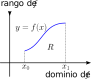
\includegraphics[scale=0.35]{figs/fig-06.pdf}
    \end{center}
    En forma similar podemos definir:
    \[ \sum_{n = 1}^{\infty} c_n = \lim_{n \rightarrow \infty} (c_1 + \cdots + c_n) \]

        Por su estructura, \textbf{son válidos} todos los teoremas usuales.

     \cw{0.3}
     En particular, si $S = \{ z: \sum a_n z^n \text{ converge } \} $, entonces pueden darse los siguientes casos:
     \begin{enumerate}[i)]
         \item $ S = \{ 0\} $.
         \item $S = \mathbb{C} $ (todos los números complejos).
         \item Existe un $R > 0$ tal que $S = \{z: |z| < R \} $, y la convergencia es absoluta e uniforme para $|z| \leq r < R$.
         \end{enumerate}
         \begin{center}
             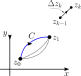
\includegraphics[scale=0.35]{figs/fig-07.pdf}
         \end{center}
 \end{columns}
\end{frame}

\begin{frame}
\begin{columns}[t]
    \cw{0.3}
    Entonces podemos \textbf{definir}:
    \begin{align*}
      e^z &= \sum_{n = 0}^{\infty} \frac{z^n}{n!} \\
      \sen z &= \sum_{n = 0}^{\infty} \frac{(-1)^n z^{2 n + 1}}{(2n +1)!} \\
     \sen x &= \sum_{n = 0}^{\infty} \frac{(-1)^n x^{2 n + 1}}{(2n +1)!} \\
    \end{align*}
    Se puede entonces probar que:
    \begin{align*}
        e^{iz} &= \cos z + i \sen z \\
               &\text{o} \\
        e^{ix} &= \cos x + i \sen x \\
        \therefore (r, \theta) &= r \cos \theta + i r \sen \theta \\
                               &= r e^{i \theta}
    \end{align*}

    \cw{0.3}
    Tres observaciones:
    \begin{enumerate}
    \item $z = r e^{i \theta} = r e^{i(\theta + 2 \pi k)} $
        \begin{align*}
        \therefore \log z &= \log r + \log e^{i(\theta + 2 \pi k)} \\
                          &= \ln r + i (\theta + 2 \pi k)
        \end{align*}
        $\therefore \log z$ es multivaluada, el \textbf{valor principal} es $-\pi < \theta \leq \pi$.
    \item 
        \begin{multline*}
            \cosh i x = \frac{e^{ix} + e^{-ix}}{2} = \\
        \frac{(\cos x + i \sen x)}{2} + \\
    \frac{\cos(-x) + i \sen(-x)}{2} = \cos x
        \end{multline*}   
\end{enumerate}

    \cw{0.3}
    \begin{enumerate}
        \setcounter{enumi}{2}
        \item $e^z = e^{x + i y} = e^x e^{iy} =$
            \begin{multline*}
            e^x (\cos y + i \sen y) = \\
            e^x \cos y + i e^x \sen y \\
            u(x, y) + i v(x, y)
            \end{multline*}
    \end{enumerate}
    $u$ y $v$ representan un \textbf{mapeo conforme} real:
    \begin{center}
        \begin{overprint}
         \onslide<1>\includegraphics[width=0.95\textwidth]{figs/fig-08.pdf}
         \onslide<2>\includegraphics[width=0.95\textwidth]{figs/fig-08b.pdf}
    \end{overprint}
    \end{center}
\end{columns}
\end{frame}

\begin{frame}{Aplicación a series ``reales''}
    \begin{columns}[c]
    \cw{0.3}
    \begin{align*}
    \frac{1}{1 - u} &= 1 + u + u^2 + \cdots \\
                    &= \sum_{n = 0}^{\infty} u^2
    \end{align*}
    converge para $|u| < 1$.
    \begin{align*}
    \therefore \frac{1}{1 + x^2} &= 1 - x^2 + x^4 - x^6 + \cdots \\
                                 &= \sum_{n}^{\infty} (-1)^n x^{2n}
    \end{align*}
    converge para $|x| < 1$.
    \cw{0.3}
    ¿Qué pasa en $x = \pm 1$?
    \begin{align*}
        \sum_{n = 0}^{\infty} (-1)^n z^{2n} &= \frac{1}{1 + z^2}, \; ({\color{red}|z| < 1}) \\
    \frac{1}{1 + z^2} &= \frac{1}{(z + i)(z -i)}
    \end{align*}
$\therefore z = \pm i \leftarrow $ \alert{¡problema!}
    \cw{0.3}
    Gráficamente:
    \begin{center}
    \includegraphics[scale=0.40]{figs/fig-09.pdf}
    \end{center}
    Los puntos problemáticos están \textbf{sobre} $|z| = 1$, pero no en $z = 1$ o en $z = -1$.
    Los puntos problemáticos están \textbf{sobre} $|z| = 1$, pero no en $z = 1$ o en $z = -1$.
    \end{columns}
\end{frame}


\begin{frame}{Integración de funciones complejas}
 \begin{columns}[t]
 
  \cw{0.35}
 
 \textbf{Revisión:}
  \[ \int_{x_0}^{x_1} f(x) \, dx = \lim_{\substack{\max \\ \Delta x \rightarrow 0}} \sum_{k=1}^n f(c_k^*) \Delta x_k \]


  \[ = F(x_1) - F(x_0), \; F' = f \]
 

  \begin{center}
      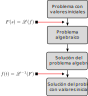
\includegraphics[width=0.85\textwidth]{figs/fig-01.pdf}
  \end{center}
  
  \cw{0.35}
  \phantom{alineación de ecuaciones}

  \[ \int_{z_0}^{z_1} f(z) \, dz \overset{{\color{red}{?}}}{=} \lim_{\substack{\max \\ \Delta z \rightarrow 0}} \sum_{k=1}^n f(c_k^*) \overset{{\color{red}{?}}}{\Delta z_k} \]

  \[ C: \begin{cases}
      x = x(t) \\
      y = y(y) \\
  \end{cases} = 
  \begin{cases}
      \vec{R} = x(t) \hat{i} + y(t) \hat{j} \\
      z = x(t) + i y(t) \\
  \end{cases} \]

   $\qquad t_0 \leq t \leq t_1$ 

   \begin{multline*} \int_{C: z_0}^{z_1} f(z) \, dz = \lim_{\substack{\max \\ \Delta z \rightarrow 0}} \sum_{k=1}^n f(c_k(t_k)) \frac{\Delta z_k}{\Delta t_k} \Delta t_k \\
       \therefore \int_{C: z_0}^{z_1} f(z) \, dz = \int_{t_0}^{t_1} f(z(t)) z'(t) \, dt
   \end{multline*}

  \cw{0.25}
  \vspace{2em}
  \begin{center}
      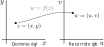
\includegraphics[width=0.85\textwidth]{figs/fig-02.pdf}
  \end{center}

\end{columns}


\end{frame}

\begin{frame}
 \begin{columns}[t]
   \cw{0.45}
   En términos de $u$ y $v$: $f(z) = u + i v$, $\Delta z = \Delta x + i \Delta y$:
   \begin{multline*}
    \int_{\substack{C \\z_0}}^{z_1} f(z) \, dz = \int_{\substack{C \\ (x_0, y_0)}}^{(x_1, y_1)} (u + i v)(dx + i dy) = \\
       \int_{\substack{C \\ (x_0, y_0)}}^{(x_1, y_1)} (u \, dx - v \, dy) + i \int_{\substack{C \\ (x_0, y_0)}}^{(x_1, y_1)} (v \, dx + u \, dy) \\
       C: \begin{cases}
           x = x(t) \\
           y = y(t)
       \end{cases}
   \end{multline*}

   Si $u + i v$ es \alert{analítica}: $u_x = v_y, \; u_y = -v_x$.

   \[ \therefore \begin{rcases*}
       u \, dx - v \, dy \\
       v \, dx + u \, dy
\end{rcases*} \text{ es diferencial exacta.} \]

   \cw{0.45}

$\therefore$ Si $f = u + i v$ en analítica:
\[ \int_{z_0}^{z_1} f(z) \, dz \]
es \textbf{independiente} de $C$, y
\[ \boxed{ \oint_C f(z) \, dz = 0, \quad \forall C} \]

$f$ analítica $\rightarrow$ 
\[ \int_{z_0}^{z_1} f(z) \, dz = F(z_1) - F(z_0), \quad F' = f \]

\begin{alertblock}{Nota:}
    \[ \oint_C f(z) \, dz \]
    \textbf{no necesariamente es 0} si $f$ no es analítica.
\end{alertblock}
\end{columns}
\end{frame}

\begin{frame}{Ejemplo}
    \begin{columns}[t]
        \cw{0.3}
        Calcular: \[ \oint_C \frac{dz}{z} \]
        donde
  \begin{center}
      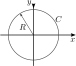
\includegraphics[width=0.75\textwidth]{figs/fig-03.pdf}
  \end{center}
  El integrando es analítico en $\mathbb{C}$ excepto en $z = 0$.

  \cw{0.3}
  Método \#1:
  \begin{multline*}
    \oint_C \frac{dz}{z} = \oint_C \frac{dx + i dy}{x + i y} \\
    = \oint_C \frac{(x-iy)(dx + i dy)}{x^2 + y^2} = \\
    \oint_C\frac{x \, dx + y \, dy}{x^2 + y^2} + i \oint_C \frac{-y \, dx + x \, dy}{x^2 + y^2}
  \end{multline*}
    En $C$: $x = R \cos \theta, \, y = R \sen \theta$, $dx = -R \sen \theta \, d\theta$, \\ $dy = R \cos \theta \, d\theta$, $x^2 + y^2 = R^2, \, 0 \leq \theta \leq 2 \pi$.
    \begin{multline*}
        \therefore \oint_C \frac{dz}{z} = 0 \\
        + i \int_0^{2 \pi} \frac{R^2(\sen^2 \theta + \cos^2 \theta) \, d\theta}{R^2} \\
        = \boxed{2 \pi i}
    \end{multline*}
  
    \cw{0.3}
    Método \#2:
    $C: z = R e^{i \theta}, \; 0 \leq \theta \leq 2 \pi$.
    \begin{multline*}
        \frac{dz}{d\theta} = i R e^{i \theta} \\
        \oint_C \frac{dz}{z} = \int_0^{2 \pi} \frac{1}{z(\theta)} \frac{dz}{d\theta} d\theta \\
    = \int_0^{2 \pi} \frac{i R e^{i \theta}}{R e^{i \theta}} d\theta \\
    = \boxed{2 \pi i}
    \end{multline*}
    \end{columns}
\end{frame}

\begin{frame}
 \begin{columns}[t]
    \cx
    Geometría elástica (topología):
  \begin{center}
      
\includegraphics[scale=0.45]{figs/fig-04.pdf}
  \end{center}

  Si $f$ es analítica en $C_1$ y $C_2$, y en la región entre ellas, entonces:
  \[ \oint_{C_1} f(z) \, dz = \oint_{C_2} f(z) \, dz \]
  \begin{center}
      
\includegraphics[scale=0.45]{figs/fig-04b.pdf}
  \end{center}

 \cx
 \[\oint_{\cancel{C}} f(z) \, dz = \oint_{C_2} f(z) \, dz - \oint_{C_1} f(z) \, dz = 0 \]

 \textbf{Ejemplo:} calcular
 \[ \oint_C \frac{dz}{dz} \]
 donde
  \begin{center}
      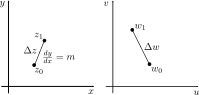
\includegraphics[scale=0.40]{figs/fig-05.pdf}
  \end{center}

  \[ \oint_C \frac{dz}{z} = \oint_{C_1} \frac{dz}{z} = 2 \pi i \]

\end{columns}
\end{frame}

\begin{frame}[standout]
    \begin{center}
        Pausa para resolver problemas de la práctica Nro. 2.

        Ejercicios 1 -- 3. 
    \end{center}
\end{frame}

\section*{Bibliografía}
\begin{frame}[allowframebreaks]{Lecturas recomendadas}
\begin{itemize}
 \item \fullcite{kreyszig2011}. Capítulo 13.
 \item \fullcite{spiegel2011}. Capítulo 1.
\end{itemize}

% \nocite{kreyszig2011}
% \nocite{spiegel2011}
% \nocite{vesely2012}
% \nocite{thornton2015}
% \printbibliography
\end{frame}


\end{document}

